\documentclass[a4paper,10pt]{article}
\usepackage[utf8]{inputenc}

% ----  Useful packages % ---- 
\usepackage{amsmath}
\usepackage{graphicx}
\usepackage{amsfonts}
\usepackage{amsthm}
\usepackage{amssymb}
\usepackage{makecell}
\usepackage{array}
\usepackage{booktabs}
\usepackage{multirow}
% ----  Useful packages % ---- 

\usepackage{wrapfig}
\usepackage{caption}
\usepackage{subcaption}
\usepackage{hyperref}
\hypersetup{
    colorlinks,
    citecolor=black,
    filecolor=black,
    linkcolor=black,
    urlcolor=black
}

\graphicspath{ {./images/} }

% ---- Set page size and margins replace ------
\usepackage[letterpaper,top=2cm,bottom=2cm,left=3cm,right=3cm,marginparwidth=1.75cm]{geometry}
% ---- Set page size and margins replace ------

% ------- NOTA ------
\theoremstyle{remark}
\newtheorem{note}{Note}[subsubsection]
% ------- NOTA ------

% ------- OSSERVAZIONE ------
\theoremstyle{definition}
\newtheorem{observation}{Osservazione}[subsection]
% ------- OSSERVAZIONE ------

% ------- DEFINIZIONE ------
\theoremstyle{plain}
\newtheorem{definition}{Definizione}[subsection]
% ------- DEFINIZIONE ------

% ------- ESEMPIO ------
\theoremstyle{definition}
\newtheorem{example}{Esempio}[subsection]
% ------- ESEMPIO ------

% ------- DIMOSTRAZIONE ------
\theoremstyle{definition}
\newtheorem{demostration}{Dimostrazione}[subsection]
% ------- DIMOSTRAZIONE ------

% ------- TEOREMA ------
\theoremstyle{definition}
\newtheorem{theorem}{Teorema}[subsection]
% ------- TEOREMA ------

% ------- COROLLARIO ------
\theoremstyle{plain}
\newtheorem{corollaries}{Corollario}[theorem]
% ------- COROLLARIO ------

% ------- PROPOSIZIONE ------
\theoremstyle{plain}
\newtheorem{proposition}{Proposizione}[subsection]
% ------- PROPOSIZIONE ------

% ---- Footer and header ---- 
\usepackage{fancyhdr}
\pagestyle{fancy}
\fancyhf{}
\fancyhead[LE,RO]{A.A 2023-2024}
\fancyhead[RE,LO]{Laboratorio II}
\fancyfoot[RE,LO]{\rightmark}
\fancyfoot[LE,RO]{\thepage}

\renewcommand{\headrulewidth}{.5pt}
\renewcommand{\footrulewidth}{.5pt}
% ---- Footer and header ---- 

% ----  Language setting ---- 
\usepackage[italian, english]{babel}
% ----  Language setting ---- 

\usepackage{listings}
\usepackage{color}

\definecolor{dkgreen}{rgb}{0,0.6,0}
\definecolor{gray}{rgb}{0.5,0.5,0.5}
\definecolor{mauve}{rgb}{0.58,0,0.82}

\lstset{frame=tb,
  language=C,
  aboveskip=3mm,
  belowskip=3mm,
  showstringspaces=false,
  columns=flexible,
  basicstyle={\small\ttfamily},
  numbers=none,
  numberstyle=\tiny\color{gray},
  keywordstyle=\color{blue},
  commentstyle=\color{dkgreen},
  stringstyle=\color{mauve},
  breaklines=true,
  breakatwhitespace=true,
  tabsize=3
}

\title{\textbf{Laboratorio II}}
\author{Realizzato da: Ghirardini Filippo}
\date{A.A. 2023-2024}

\begin{document}
\begin{titlepage} %crea l'enviroment
	\begin{figure}[t] %inserisce le figure
		\centering
\includegraphics[width=0.98\textwidth]{marchio_unipi_pant541.png}
	\end{figure}
	\vspace{20mm}
	
	\begin{Large}
		\begin{center}
			\textbf{Dipartimento di Informatica\\ Corso di Laurea Triennale in Informatica\\}
			\vspace{20mm}
			{\LARGE{Corso a Libera Scelta - 6 CFU}}\\
			\vspace{10mm}
			{\huge{\bf Computer Graphics}}\\
		\end{center}
	\end{Large}
	
	
	\vspace{36mm}
	%minipage divide la pagina in due sezioni settabili
	\begin{minipage}[t]{0.47\textwidth}
		{\large{\bf Professore:}\\ \large{Prof. }}
	\end{minipage}
	\hfill
	\begin{minipage}[t]{0.47\textwidth}\raggedleft
		{\large{\bf Autore:}\\ \large{Filippo Ghirardini}}
	\end{minipage}
	
	\vspace{25mm}
	
	\hrulefill
	
	\vspace{5mm}
	
	\centering{\large{\bf Anno Accademico 2023/2024 }}
	
\end{titlepage}

\tableofcontents
\newpage
\maketitle
\begin{center}
    \vspace{-20pt}
    \rule{11cm}{.1pt} 
\end{center}
\newpage
% !TeX spellcheck = it_IT
\section{Thread}
Ci garantiscono di avere più unità di calcolo a disposizione all'interno del nostro programma. Non si pone più il problema della comunicazione, in quanto è tutto in comune, ma anzi adesso bisogna evitare che i dati si diano fastidio.\\
\href{https://man7.org/linux/man-pages/man7/pthreads.7.html}{Link alla pagina del manuale per pthreads.}\\
Esistono due tipologie di thread:
\begin{itemize}
	\item \textbf{Joinable}: ci si aspetta che il thread principale esegua una join
	\item \textbf{Detached}: sono pensati per essere lanciati e ignorati dal thread principale. Quando terminano non rimangono \emph{zombie}
\end{itemize}

\begin{example}[Conta primi]
	\label{example:threads_prime}
	\begin{lstlisting}[language=C]
		#include "xerrori.h"
		// Prototipi
		bool primo(int n);
		
		// Struct che uso per passare argomenti ai thread
		typedef struct {
			int start;            // intervallo dove cercare i primo 
			int end;              // parametri di input
			int somma_parziale;   // parametro di output
		} dati;
		
		// Funzione passata a pthred_create
		void *tbody(void *v) {
			dati *d = (dati *) v;
			int primi = 0;
			// Cerco i primi nell'intervallo assegnato
			for(int j=d->start;j<d->end;j++) {
				if(primo(j)) primi++; 
				usleep(1);
			}
			fprintf(stderr, "Il thread che partiva da %d ha terminato\n", d->start);
			d->somma_parziale = primi;
			pthread_exit(NULL);
		}
		
		int main(int argc,char *argv[])
		{
			if(argc!=3) {
				fprintf(stderr,"Uso\n\t%s m num_threads\n", argv[0]);
				exit(1);
			}
			// conversione input
			int m= atoi(argv[1]);
			if(m<1) termina("limite primi non valido");
			int p= atoi(argv[2]);
			if(p<=0) termina("numero di thread non valido");
			
			// creazione thread ausiliari
			pthread_t t[p];   // Array di p indentificatori di thread 
			dati d[p];        // Array di p struct che passero ai p thread
			int somma = 0;        // Variabile dove accumulo il numero di primi
			for(int i=0; i<p; i++) {
				int n = m/p;  // Quanti numeri verifica ogni thread + o - 
				d[i].start = n*i; // Inizio range thread i
				d[i].end = (i==p-1) ? m : n*(i+1);
				xpthread_create(&t[i], NULL, &tbody, &d[i],__LINE__, __FILE__); 
			}
			// Attendo che i thread abbiano finito
			for(int i=0;i<p;i++) {
				xpthread_join(t[i],NULL,__LINE__, __FILE__);
				somma += d[i].somma_parziale;
			}
			// Restituisce il risultato 
			printf("Numero primi tra 1 e %d (escluso): %d\n",m,somma);
			return 0;
		}
	\end{lstlisting}
\end{example}

\subsection{Creazione}
La funzione utilizzata \emph{xpthreads} è un'estensione di \emph{pthreads} con la gestione degli errori, e prende in input i seguenti parametri:
\begin{enumerate}
	\item L'\textbf{indirizzo} nel quale verrà scritto un identificatore per il thread
	\item Eventuali \textbf{caratteristiche speciali} (non ci serve nel corso)
	\item La \textbf{funzione} che contiene il codice eseguito dal thread
	\item  Ciò che viene dato come \textbf{argomento} alla funzione passata come terzo argomento. Essendo \emph{void} andrà fatto un \textbf{casting} con le conseguenti precauzioni
\end{enumerate}
Nell'esempio \ref{example:threads_prime}, non abbiamo rischi di \textbf{condivisione} di valori in quanto ogni thread ha solo accesso alla funzione che gli passiamo e con essa i parametri ed eventuali variabili globali (che non andrebbero mai utilizzate).

\subsection{Chiusura}
Per la terminazione di un thread si può chiamare
\begin{lstlisting}[language=C]
	pthread_exit(NULL);
\end{lstlisting}
o alternativamente
\begin{lstlisting}[language=C]
	return(NULL);
\end{lstlisting}
È possibile restituire alla funzione principale dei dati ma per il nostro tipo di utilizzo gestiremo lo scambio di informazioni tramite passaggi di indirizzo, senza ritornare nulla.

\subsection{Attesa}
Per attendere la terminazione di un thread si utilizza
\begin{lstlisting}[language=C]
	xpthread_join(t[i],NULL,__LINE__,__FILE__);
\end{lstlisting}
che prende in input l'identificatore del thread in questione. Il secondo parametro serve eventualmente per recuperare ciò che mi viene restituito (noi quindi non lo utilizziamo).

\subsection{Errore}
La gestione degli errori è implementata dal professore come segue
\begin{lstlisting}[language=C]
	#define Buflen 100
	void xperror(int en, char *msg) {
		char buf[Buflen];
		
		char *errmsg = strerror_r(en, buf, Buflen);
		if(msg!=NULL)
		fprintf(stderr,"%s: %s\n",msg, errmsg);
		else
		fprintf(stderr,"%s\n",errmsg);
	}
	
	int xpthread_create(pthread_t *thread, const pthread_attr_t *attr,
	void *(*start_routine) (void *), void *arg, int linea, char *file) {
		int e = pthread_create(thread, attr, start_routine, arg);
		if (e!=0) {
			xperror(e, "Errore pthread_create");
			fprintf(stderr,"== %d == Linea: %d, File: %s\n",getpid(),linea,file);
			pthread_exit(NULL);
		}
		return e;                       
	}
	
	int xpthread_join(pthread_t thread, void **retval, int linea, char *file) {
		int e = pthread_join(thread, retval);
		if (e!=0) {
			xperror(e, "Errore pthread_join");
			fprintf(stderr,"== %d == Linea: %d, File: %s\n",getpid(),linea,file);
			pthread_exit(NULL);
		}
		return e;
	}
\end{lstlisting}
Dato che i thread condividono le variabili globali, non possiamo sfruttare \emph{errno} come con le altre funzioni. Viene quindi utilizzato il valore di ritorno della \emph{create} e della \emph{join}.

\begin{note}
	Alcuni comandi aggiuntivi:
	\begin{lstlisting}[language=C]
		gettid(); // Restituisce l'ID del thread
	\end{lstlisting}
\end{note}

\subsection{Implementazione}
\begin{example}[Tabella numeri primi]
	\label{example:primetable}
	\begin{lstlisting}[language=C]
		#include "xerrori.h"
		#define QUI __LINE__, __FILE__
		
		//Prototipi
		bool primo(int n);
		
		// struct che uso per passare argomenti ai thread
		typedef struct {
			int start;            // intervallo dove cercare i primo 
			int end;              // parametri di input
			int somma_parziale;   // parametro di output
			int *tabella;         // tabella dei numeri primi da riempire
			int *pmessi;          // puntatore a indice in tabella
			pthread_mutex_t *pmutex; // mutex condiviso
		} dati;
		
		// funzione passata a pthred_create
		void *tbody(void *v) {
			dati *d = (dati *) v;
			int primi = 0;
			// cerco i primi nell'intervallo assegnato
			for(int j=d->start;j<d->end;j++)
			if(primo(j)) {
				primi++;
				xpthread_mutex_lock(d->pmutex,QUI);
				d->tabella[*(d->pmessi)] = j;
				*(d->pmessi) += 1;
				xpthread_mutex_unlock(d->pmutex,QUI);
			}
			fprintf(stderr, "Il thread che partiva da %d ha terminato\n", d->start);
			d->somma_parziale = primi;
			pthread_exit(NULL);
		}
		
		int main(int argc,char *argv[])
		{
			if(argc!=3) {
				fprintf(stderr,"Uso\n\t%s m num_threads\n", argv[0]);
				exit(1);
			}
			// conversione input
			int m= atoi(argv[1]);
			if(m<1) termina("limite primi non valido");
			int p= atoi(argv[2]);
			if(p<=0) termina("numero di thread non valido");
			
			// definizione mutex
			pthread_mutex_t mtabella;
			xpthread_mutex_init(&mtabella,NULL,QUI);
			// creazione thread ausiliari
			pthread_t t[p];   // array di p indentificatori di thread 
			dati d[p];        // array di p struct che passero allle p thread
			int somma = 0;        // variabile dove accumulo il numero di primi
			int *tabella = malloc(m*sizeof(int));
			if(tabella==NULL) xtermina("Allocazione fallita", __LINE__, __FILE__);
			int messi = 0;
			for(int i=0; i<p; i++) {
				int n = m/p;  // quanti numeri verifica ogni figlio + o - 
				d[i].start = n*i; // inizio range figlio i
				d[i].end = (i==p-1) ? m : n*(i+1);
				d[i].tabella = tabella;
				d[i].pmessi = &messi;
				d[i].pmutex = &mtabella;
				xpthread_create(&t[i], NULL, &tbody, &d[i],__LINE__, __FILE__); 
			}
			// attendo che i thread abbiano finito
			for(int i=0;i<p;i++) {
				xpthread_join(t[i],NULL,__LINE__, __FILE__);
				somma += d[i].somma_parziale;
			}
			xpthread_mutex_destroy(&mtabella,QUI);
			// stampa tabella
			for(int i=0;i<messi;i++)  printf("%8d",tabella[i]);
			printf("\nPrimi in tabella: %d\n",messi);
			// restituisce il numero di primi
			printf("Numero primi tra 1 e %d (escluso): %d\n",m,somma);
			return 0;
		}
	\end{lstlisting}
\end{example}

\begin{note}
	Il tipo di dato da noi definito, avrà anche il numero di primi inseriti. Questo deve necessariamente essere un puntatore poiché deve essere condiviso tra tutti i thread e altrimenti ce ne sarebbe uno diverso per ognuno.
\end{note}
\subsubsection{Mutex}
Per garantire l'accesso da parte di più thread ad un'unica risorsa in memoria è necessario usare i \textbf{mutex} (andrebbero bene anche i semafori). In questo modo permettiamo l'accesso \emph{esclusivo} ad un solo thread alla volta.\\
Un mutex può avere due stati: \textbf{locked} e \textbf{unlocked}. Quando un thread ha bisogno della risorsa associata, lo blocca, accede alla risorsa e poi lo sblocca. Se un altro thread nel frattempo prova ad accedere rimane in attesa che si sblocchi il mutex.\\
La \textbf{creazione} del mutex avviene come segue:
\begin{lstlisting}[language=C]
	pthread_mutex_t mutex;
	xpthread_mutex_init(&mutex,NULL,__LINE__,__FILE__);
\end{lstlisting}
Anche qui il secondo parametro serve per specificare eventuali caratteristiche che deve avere il mutex. Le \textbf{operazioni} su di esso si fanno come segue:
\begin{lstlisting}[language=C]
	xpthread_mutex_lock(mutex,__LINE__,__FILE__);
	xpthread_mutex_unlock(mutex,__LINE__,__FILE__);
	xpthread_mutex_destroy(&mutex,__LINE__,__FILE__);
\end{lstlisting}

\begin{note}
	\label{note:mutex_efficiency}
	È importante sbloccare il \emph{mutex} il prima possibile per evitare attese inutili e garantire l'efficienza del codice.
\end{note}

\subsubsection{Semafori}
Abbiamo un compito complesso da eseguire, che consiste in una serie di \emph{task} ognuno suddiviso in due parti A e B. Prima di eseguire la parte B devo necessariamente aver eseguito la parte A ma mentre eseguo la B posso iniziare ad eseguire il task successivo.
\begin{center}
	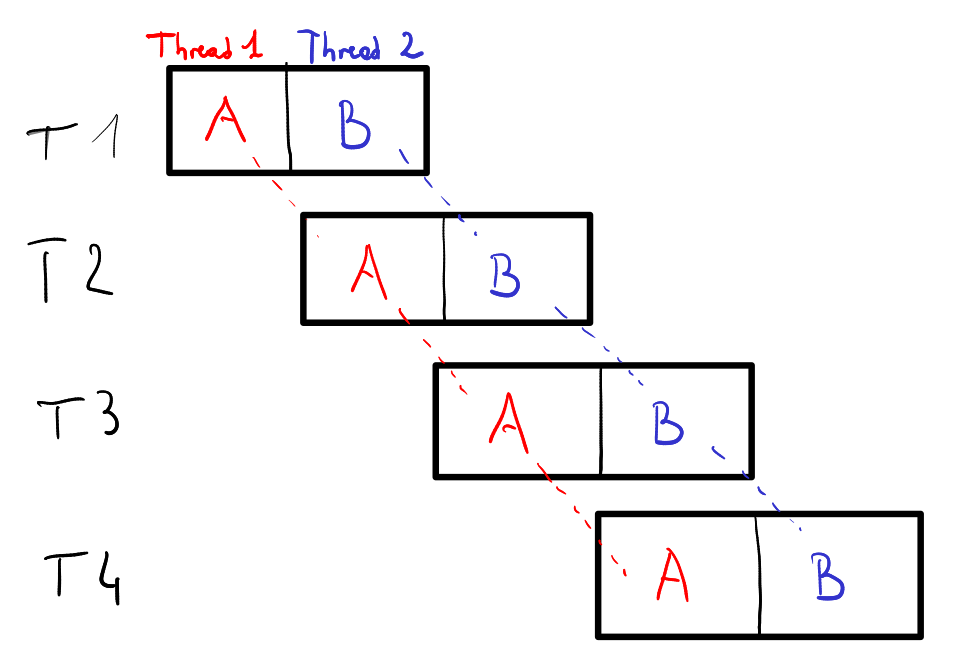
\includegraphics[scale=0.3]{prod_cons.png}
\end{center}
Tutte le parti A del task verranno eseguite dal thread 1 (\textbf{produttore}) e tutte le B dal 2 (\textbf{consumatore}). Di conseguenza se ogni parte richiede $1u$ di tempo, con questo schema serviranno $5u$.\\
Si rende necessario un modo di condividere le informazioni tra i due thread, ovvero condividere i risultati della parte A. Il secondo thread di contro deve rimanere in attesa finché non gli arrivano i risultati da poter elaborare nella parte B.\\
Per fare ciò si usano i \textbf{semafori}, in modo che il secondo thread rimanga in \textbf{wait} in attesa dei dati, e appena il primo ha finito di lavorare mette i dati nel buffer comune e fa una \textbf{post} che sblocca il secondo.\\
Questo meccanismo è utile anche considerando che non tutte le parti dei task siano effettivamente di durata uguale. In questa casistica quando il primo thread si porta avanti e arriva a calcolare il terzo task , deve mettersi in attesa per evitare di sovrascrivere il terzo risultato sopra al secondo che non è ancora stato elaborato.
\begin{center}
	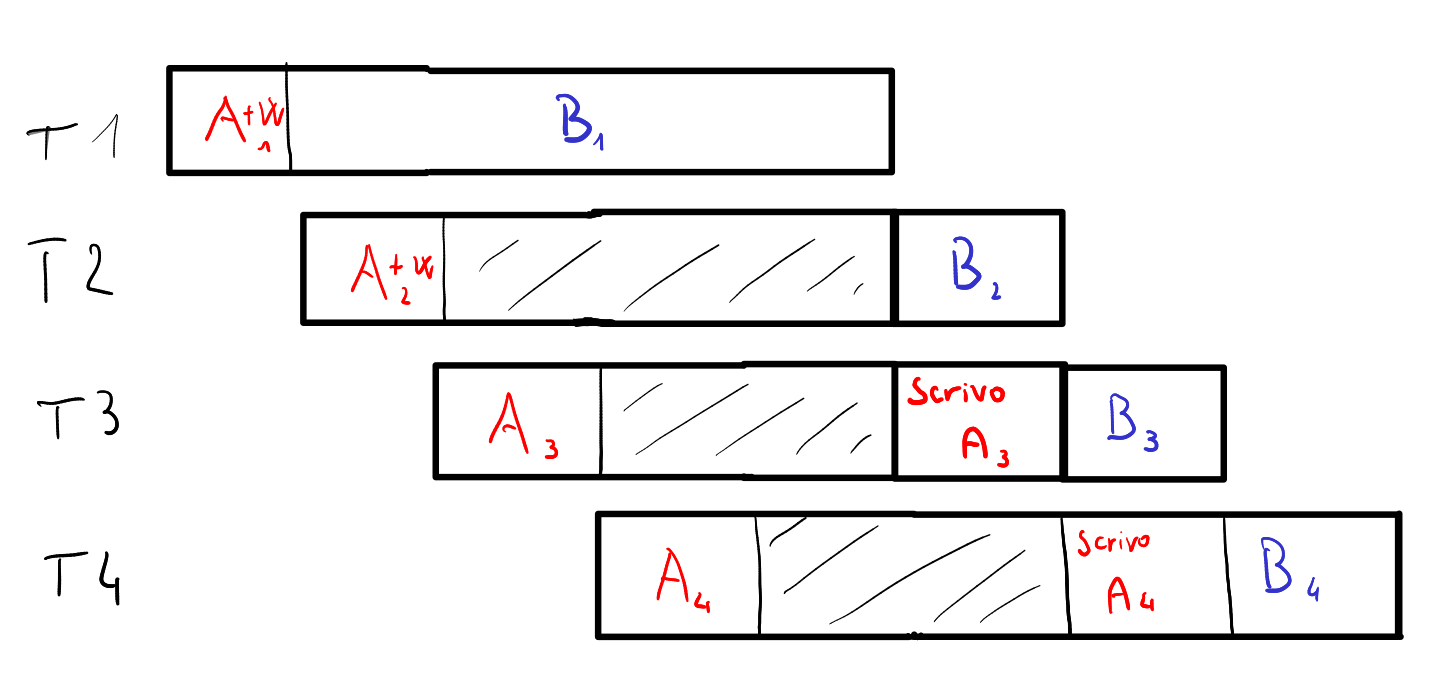
\includegraphics[scale=0.3]{prod_cons_2.png}
\end{center}
\begin{example}
	Esempio di esecuzione di 8 task con le varie fasi:
	\begin{table}[!h]
		\centering
		\begin{tabular}{|c|c|c|c|c|c|c|c|c|}
			\hline
			\textbf{\#Task} & \textbf{1} & \textbf{2} & \textbf{3} & \textbf{4} & \textbf{5} & \textbf{6} & \textbf{7} & \textbf{8} \\
			\hline
			Inizio calcolo & 0 & 2 & 3 & 4 & 5 & 6 & 7 & 8\\
			Tempo prod & 2 & 1 & 1 & 1 & 1 & 1 & 1 & 1 \\
			Fine calcolo prod & 2 & 3 & 4 & 5 & 6 & 7  &8  &9 \\
			Scrittura buffer & 2 & 3 & 4 & 5 & 6 & 7  &8  &9 \\
			Lettura cons & 2 & 3 & 4 & 5 & 6 & 7  &8  &9 \\
			Tempo cons& 1 & 1 & 1 & 1 & 1 & 1 & 1 & 1 \\
			Fine totale & 3 & 4 & 5 & 6 & 7  &8  &9 & 10 \\
			\hline
		\end{tabular}
	\end{table}
	Se cambiamo i tempi necessari al produttore e al consumatore:
	\label{example:prodcons}
	\begin{table}[!h]
		\centering
		\begin{tabular}{|c|c|c|c|c|c|c|c|c|}
			\hline
			\textbf{\#Task} & \textbf{1} & \textbf{2} & \textbf{3} & \textbf{4} & \textbf{5} & \textbf{6} & \textbf{7} & \textbf{8} \\
			\hline
			Inizio calcolo & 0 & 1 & 2 & 6 & 11 &16 & 21 & 26\\
			Tempo prod & 1 & 1 & 1 & 1 & 5 & 5 & 5 & 5 \\
			Fine calcolo prod & 1 & 2& 3 & 7 & 16 & 21  &26  &31 \\
			Scrittura buffer & 1 & 2 & 6 & 11 & 16 & 21  &26  &31 \\
			Lettura cons & 1 & 6 & 11 & 16 & 21 & 22  &26  &31 \\
			Tempo cons& 5 & 5 & 5 & 5 & 1 & 1 & 1 & 1 \\
			Fine totale & 6 & 11 & 16 & 21 & 22  &23  &27 & 32 \\
			\hline
		\end{tabular}
	\end{table}
	In questo caso abbiamo delle inefficienze in quanto produttore e consumatore devono aspettarsi a vicenda avendo tempistiche di lavoro diverse.
\end{example}
Per risolvere il problema descritto nell'esempio \ref{example:prodcons} è possibile aumentare la \textbf{grandezza del buffer}, permettendo di accumulare più di un singolo risultato della parte A alla volta e riducendo quindi i tempi.\\
Per implementare la soluzione usiamo due semafori:
\begin{itemize}
	\item \textbf{sem\_free\_slots}, inizializzato a $b$, indica il numero di slot dove il produttore può scrivere
	\item \textbf{sem\_data\_items}, inizializzato a $0$, indica il numero di oggetti scritti dal produttore che il consumatore deve elaborare
\end{itemize}
Se il produttore deve scrivere qualcosa effettua
\begin{lstlisting}[language=C]
	sem_wait(sem_free_slots);
\end{lstlisting}
e dopo aver aspettato effettua la scrittura del dato e poi
\begin{lstlisting}[language=C]
	sem_post(sem_data_items);
\end{lstlisting}
Quando invece il consumatore vuole un nuovo dato effettua
\begin{lstlisting}[language=C]
	sem_wait(sem_data_items);
\end{lstlisting}
che aspetta che ci sia un dato disponibile e mantiene aggiornato il numero di oggetti sul buffer. Legge poi il dato ed esegue
\begin{lstlisting}[language=C]
	sem_post(sem_free_slots);
\end{lstlisting}
che mantiene aggiornato il numero di slot liberi.\\
Dopo ogni operazione è mantenuto l'invariante:
\begin{equation*}
	sem\_free\_slots + sem\_data\_items = b
\end{equation*}
Per gestire le posizioni libere occupate nel buffer usiamo un indice $p$ per la prossima posizione dove scriverà il produttore e un indice $c$ per la prossima posizione dove legge il consumatore.\\
Grazie all'uso dei semafori abbiamo che:
\begin{equation*}
	c \leq p \leq c+b
\end{equation*}
Quando $c=p$, sem\_data\_items vale $0$ e $c$ non può avanzare oltre, quando invece $p=c+b$, sem\_free\_slots è $0$ e $p$ non può avanzare oltre. In questo modo facciamo finta di avere un buffer infinito ma accediamo alle posizioni $c\%b$ e $p\%b$ che sono tra $0$ e $b-1$.
\begin{example}
	Modifichiamo l'esempio \ref{example:threads_prime} implementando un buffer e dei semafori.
	\label{example:semafori}
	\begin{lstlisting}[language=C]
		#define Buf_size 10
		
		// Struct contenente i parametri di input e output di ogni thread 
		typedef struct {
			int quanti;   // output
			long somma;   // output
			int *buffer; 
			int *pcindex;
			sem_t *sem_free_slots;
			sem_t *sem_data_items;  
		} dati;
		
		// Funzione eseguita dai thread consumer
		void *tbody(void *arg)
		{  
			dati *a = (dati *)arg; 
			a->quanti = 0;
			a->somma = 0;
			int n;
			fprintf(stderr,"Consumatore %d partito\n",gettid());
			do {
				xsem_wait(a->sem_data_items,__LINE__,__FILE__);
				n = a->buffer[*(a->pcindex) % Buf_size];
				*(a->pcindex) +=1;
				xsem_post(a->sem_free_slots,__LINE__,__FILE__);
				if(n>0 && primo(n)) {
					a->quanti++;
					a->somma += n;
				}
			} while(n!= -1);
			fprintf(stderr,"Consumatore %d sta per terminare\n",gettid());
			pthread_exit(NULL); 
		}     
		
		int main(int argc, char *argv[])
		{
			// Leggi input
			if(argc!=2) {
				printf("Uso\n\t%s file\n", argv[0]);
				exit(1);
			}
			// Numero di thread ausiliari 
			int p = 1;
			assert(p>0);
			int tot_primi = 0;
			long tot_somma = 0;
			int e,n,cindex=0;    
			// Threads related
			int buffer[Buf_size];
			int pindex=0;
			// pthread_mutex_t mu = PTHREAD_MUTEX_INITIALIZER;
			pthread_t t[p];
			dati a[p];
			sem_t sem_free_slots, sem_data_items;
			xsem_init(&sem_free_slots,0,Buf_size,__LINE__,__FILE__);
			xsem_init(&sem_data_items,0,0,__LINE__,__FILE__);
			for(int i=0;i<p;i++) {
				// Faccio partire il thread i
				a[i].buffer = buffer;
				a[i].pcindex = &cindex;
				a[i].sem_data_items = &sem_data_items;
				a[i].sem_free_slots = &sem_free_slots;
				xpthread_create(&t[i],NULL,tbody,a+i,__LINE__,__FILE__);
			}
			fputs("Thread ausiliari creati\n",stderr);
			FILE *f = fopen(argv[1],"r");
			if(f==NULL) {perror("Errore apertura file"); return 1;}
			while(true) {
				e = fscanf(f,"%d", &n);
				if(e!=1) break; // Se il valore letto correttamente e==1
				assert(n>0);    // I valori del file devono essere positivi
				xsem_wait(&sem_free_slots,__LINE__,__FILE__);
				buffer[pindex++ % Buf_size]= n;
				xsem_post(&sem_data_items,__LINE__,__FILE__);
			}
			fputs("Dati del file scritti nel buffer\n",stderr);
			if(fclose(f)!=0) xtermina("Errore chiusura input file",__LINE__,__FILE__);
			// Terminazione threads
			for(int i=0;i<p;i++) {
				xsem_wait(&sem_free_slots,__LINE__,__FILE__);
				buffer[pindex++ % Buf_size]= -1;
				xsem_post(&sem_data_items,__LINE__,__FILE__);
			}
			fputs("Valori di terminazione scritti nel buffer\n",stderr);
			// Join dei thread e calcolo risultato
			for(int i=0;i<p;i++) {
				xpthread_join(t[i],NULL,__LINE__,__FILE__);
				tot_primi += a[i].quanti;
				tot_somma += a[i].somma;
			}
			xsem_destroy(&sem_data_items,__LINE__,__FILE__);
			xsem_destroy(&sem_free_slots,__LINE__,__FILE__);
			// pthread_mutex_destroy(&mu);
			printf("Trovati %d primi con somma %ld\n",tot_primi,tot_somma);
			return 0;
		}
	\end{lstlisting}
\end{example}
\begin{note}
	Come visto in \ref{note:mutex_efficiency} è importante dare il via libera agli altri thread tramite una \emph{post} del semaforo il prima possibile per garantire l'efficienza del codice.
\end{note}
Il problema di questo metodo è la \textbf{terminazione}. La strategia più semplice per segnalare al consumatore che il lavoro è finito è quello di passare un valore \emph{dummy} concordato in precedenza. Ad esempio nel caso \ref{example:semafori} abbiamo usato $-1$.

\begin{observation}
	Se invece di utilizzare un buffer di tipo circolare utilizzassi una pila, non sarebbe garantito l'ordine di elaborazione dei dati prodotti dei dati dal consumatore, che potrebbe trovarsi come primo dato il \emph{dummy} e terminare subito.
\end{observation}

\subsubsection{Condition variables}
Ci permette di utilizzare condizioni per fermare il thread personalizzate.
\begin{example}
	Supponiamo di avere diversi thread che eseguono diverse operazioni, ognuna con una necessità di memoria diversa. Il sistema ha a disposizione $100MB$ da dividere tra di loro. Si rende quindi necessario un controllore centrale che gestisca la cessione della memoria ai vari thread.\\
	Se ad esempio un primo thread richiede $20MB$, i disponibili diventano $80MB$. Quando poi un altro thread ne richiede ad esempio $90MB$, il controllore deve metterlo in attesa finché non ne sono disponibili di nuovo a sufficienza.
	\begin{lstlisting}
		fprintf(stderr,"%2d Assegnati: %3d. Rimanenti: %4d\n\n", gettid()%100,
		memoria_disponibile >= quante_ne_serve
	\end{lstlisting}
\end{example}
La comodità rispetto ai semafori è che in questi l'unico test possibile è verificare che il suo valore sia $\geq 0$ mentre in questo caso non siamo vincolati.\\
Una possibile implementazione è la seguente:
\begin{lstlisting}[language=C]
	// Struct che tiene traccia della memoria disponibile e 
	// contiene le variabili cond/mutex per regolarne l'utilizzo
	typedef struct {
		pthread_cond_t  *cv; // Condition variable
		pthread_mutex_t *mu; // Mutex
		int MB;       // Memoria attualmente disponibile
	} heap;
	
	// Simula allocazione con spazio limitato
	void richiedi(heap *h, int n) {
		// E' necessario che anche il ciclo while sia sotto lock del mutex
		xpthread_mutex_lock(h->mu,QUI);
		while(n>h->MB) {
			// In automatico viene rilasciato il mutex prima di addormentarsi
			xpthread_cond_wait(h->cv,h->mu,QUI);
			// Al risveglio del thread viene riacquisito il mutex (se ce ne sono diversi in attesa, il piu veloce lo prende, gli altri attendono)
		}
		h->MB -= n;
		xpthread_mutex_unlock(h->mu,QUI);
	}
	
	// Deallocazione
	void libera(heap *h, int n) {
		xpthread_mutex_lock(h->mu,QUI);
		h->MB += n;
		// Sveglia tutti i thread avvisando che ci sono risorse disponibili
		xpthread_cond_broadcast(h->cv,QUI);
		xpthread_mutex_unlock(h->mu,QUI); 
	}
	
	// Codice thread tipo 1, chiede 10,20,...,50
	void *tipo1(void *v) {
		heap *h = (heap *) v;
		for(int i=1;i<=5;i++) {
			int m = 10*i;
			richiedi(h,m);
			sleep(1);
			libera(h,m);
		}
		return NULL;
	}
	
	// Codice thread tipo 2, chiede 15,25,...,55
	void *tipo2(void *v) {
		heap *h = (heap *) v;
		for(int i=1;i<=5;i++) {
			int m = 10*i+5;
			richiedi(h,m);
			sleep(1);
			libera(h,m);
		}
		return NULL;
	}
	
	int main(int argc, char *argv[])
	{		
		// Inizializza heap 
		pthread_cond_t c = PTHREAD_COND_INITIALIZER;
		pthread_mutex_t m = PTHREAD_MUTEX_INITIALIZER;
		heap h;
		h.cv = &c; h.mu = &m;
		h.MB = mem;
		
		// Esegue i thread
		pthread_t t[nt];
		// Esegue un thread tipo1
		xpthread_create(&t[0],NULL,&tipo1,&h,QUI);
		for(int i=1;i<nt;i++)
		// Esegue nt-1 thread di tipo 2
			xpthread_create(&t[i],NULL,&tipo2,&h,QUI);
		
		// Attende terminazione thread e termina
		for(int i=0;i<nt;i++)
			xpthread_join(t[i],NULL,QUI);
		xpthread_cond_destroy(&c,QUI);
		xpthread_mutex_destroy(&m,QUI);
		
		return 0;
	}
\end{lstlisting}

\begin{example}
	Un esempio di implementazione di una soluzione al problema dei \textbf{produttori e consumatori} usando le variabili condivise è la seguente:
	\begin{lstlisting}[language=C]
		typedef struct {
			int readers;
			bool writing;
			pthread_cond_t cond;   // Condition variable
			pthread_mutex_t mutex; // Mutex associato alla condition variable
		} rw;
		
		// Inizializza rw, ne scrittori ne lettori 
		void rw_init(rw *z)
		{
			z->readers = 0;
			z->writing = false;
			xpthread_cond_init(&z->cond,NULL,QUI);
			xpthread_mutex_init(&z->mutex,NULL,QUI);
		}
		
		// Inizio uso da parte di un reader
		void read_lock(rw *z)
		{
			pthread_mutex_lock(&z->mutex);
			while(z->writing==true)
			pthread_cond_wait(&z->cond, &z->mutex);   // attende fine scrittura
			z->readers++;
			pthread_mutex_unlock(&z->mutex);
		}
		
		// Fine uso da parte di un reader
		void read_unlock(rw *z)
		{
			assert(z->readers>0);  // Ci deve essere almeno un reader (me stesso)
			assert(!z->writing);   // Non ci devono essere writer 
			pthread_mutex_lock(&z->mutex);
			z->readers--;                  // Cambio di stato       
			if(z->readers==0) 
			// A differenza della broadcast, la signal sveglia solamente uno dei thread in attesa
			pthread_cond_signal(&z->cond); 
			pthread_mutex_unlock(&z->mutex);
		}
		
		// Inizio uso da parte di writer  
		void write_lock(rw *z)
		{
			pthread_mutex_lock(&z->mutex);
			while(z->writing || z->readers>0)
			// Attende fine scrittura o lettura
			pthread_cond_wait(&z->cond, &z->mutex);   
			z->writing = true;
			pthread_mutex_unlock(&z->mutex);
		}
		
		// Fine uso da parte di un writer
		void write_unlock(rw *z)
		{
			assert(z->writing);
			pthread_mutex_lock(&z->mutex);
			z->writing=false;               // Cambio stato
			// Segnala a tutti quelli in attesa 
			pthread_cond_broadcast(&z->cond);  
			pthread_mutex_unlock(&z->mutex);
		}
	\end{lstlisting}
\end{example}
% !TeX spellcheck = it_IT
\newpage
\section{Socket}
Permettono la comunicazione tra due processi su macchine diverse. Funzionano in maniera analoga alle \textit{pipe}, quindi deve essere chiaro il \textbf{formato} con il quale vengono inviati i dati.\\
La complicazione principale delle socket è che il mezzo di trasmissione (\textbf{internet}) non è sempre disponibile e la connessione potrebbe cadere. Inoltre, a differenza delle pipe, il server interagisce con più client.

\subsection{Implementazione}
Nel corso verrà utilizzato Python perché più veloce da scrivere e comunque molto simile ai comandi in C. La differenza principale tra i due linguaggi sta nel server, che però a livello concettuale non è complesso (solo lungo).
\subsubsection{Server}
Una possibile implementazione di un \textbf{echo-server} in Python è la seguente:
\begin{lstlisting}[language=Python]
	import socket
	
	# Specifica da dove accettare le connessioni
	HOST = "127.0.0.1"  # Standard loopback interface address (localhost)
	PORT = 65432  # Port to listen on (non-privileged ports are > 1023)
	
	# Creazione del server socket
	with socket.socket(socket.AF_INET, socket.SOCK_STREAM) as s:
		s.bind((HOST, PORT)) # Accetta connessioni da HOST in riferimento alla porta PORT
		s.listen() # In ascolto
		while True:
			# In attesa di una connessione
			conn, addr = s.accept()
			# Lavoro con la connessione appena ricevuta 
			with conn:
				while True:
					data = conn.recv(64) # Leggo fino a 64 bytes
					# Se ricevo 0 bytes, termino la connessione
					if not data:
						break
					conn.sendall(data) # Altrimenti rispedisco i dati indietro
\end{lstlisting}

\subsubsection{Client}
Una possibile implementazione di un \textbf{echo-client} in Python è la seguente:
\begin{lstlisting}[language=Python]
	import sys,socket
	
	# Valori verso cui connettersi 
	HOST = "127.0.0.1" # Server hostname or IP address
	PORT = 65432 # Port used by the server

	# Creazione del socket per la connesssione al server
	with socket.socket(socket.AF_INET, socket.SOCK_STREAM) as s:
		# Mi connetto
		s.connect((host, port))
		while True:
			n = int(input("Quanti byte? "))
			if n<=0:
				break
			# Invio stringa di n a e attendo la risposta   
			msg = "a"*n
			s.sendall(msg.encode())
			data = s.recv(64)
			if len(data)==0:
				break
		# Comunico al server di chiudere la connessione
		# SHUT_RDWR indica che terminiamo sia lettura che scrittura     
		s.shutdown(socket.SHUT_RDWR)
\end{lstlisting}

\begin{observation}[Client multipli]
	Cosa succede se un altro client prova a connettersi mentre c'è già una connessione attiva?\\
	Il server stabilisce la connessione ma non risponde ad entrambi, solo ad uno, l'altro rimarrà in attesa.
\end{observation}
\begin{observation}[Violazione del protocollo]
	Cosa succede se ignoro le specifiche che mi sono dato sul formato dei dati?\\
	Si perde la sincronizzazione. Per garantirla si può ad esempio precedere i dati con la lunghezza del pacchetto.
\end{observation}
\begin{observation}[Codifica]
	In Python possiamo codificare una stringa tramite la seguente istruzione:
	\begin{lstlisting}[language=Python]
		s = "hello world"
		s.encode()
	\end{lstlisting}
	Di default utilizza la codifica \textit{UTF-8} che per i caratteri standard usa un byte mentre per quelli più complessi (e.g. €) ne usa di più. \\
	Per quanto riguarda i numeri posso scegliere il tipo di codifica tra \textit{big-endian} (!) o \textit{little-endian}:
	\begin{lstlisting}[language=Python]
		encoded = struct.pack("i", 33) # Little endian
		struct.pack("!i", 33) # Big endian
	\end{lstlisting}
	E poi per decodificarlo:
	\begin{lstlisting}[language=Python]
		struct.unpack("i", encoded)
	\end{lstlisting}
\end{observation}
\subsection{Client multipli}
Per gestire più client contemporaneamente, esistono due tipi di implementazione:
\begin{itemize}
	\item Il singolo server alterna la connessione tra i vari client
	\item Quando arriva un client, crea un \textbf{thread} dedicato a quella connessione
\end{itemize}
\end{document}
